%%%%%%%%%%%%%%%%%%%%%%%%%%%%%%%%%%%%%%%%%%%%%%%%%%%%%%%%%%%%%%%%%%%%%%%%%%%%%%
\newpage
\section {Reconstruction }

Distributions of the reconstructed track momentum and T0 for all reconstructed positive
tracks from $\pi^+ \to e^+ \nu $ decays in the ST are shown in Figure~\ref{fig:all_tracks_p_t0}.
The distributions corresponding to different degrader thicknesses are overlaid.
One can see that the probability per POT to have a reconstructed positron track reaches its maximum
for degrader thicknesses of about 2-3 mm Ti, and it starts falling down as the degrader thickness
increases.

Compared to ``no degrader'', a 2-3mm thick Ti degrader increases the acceptance by a factor
close to x3.

\begin{figure}[H]
  % \centering
  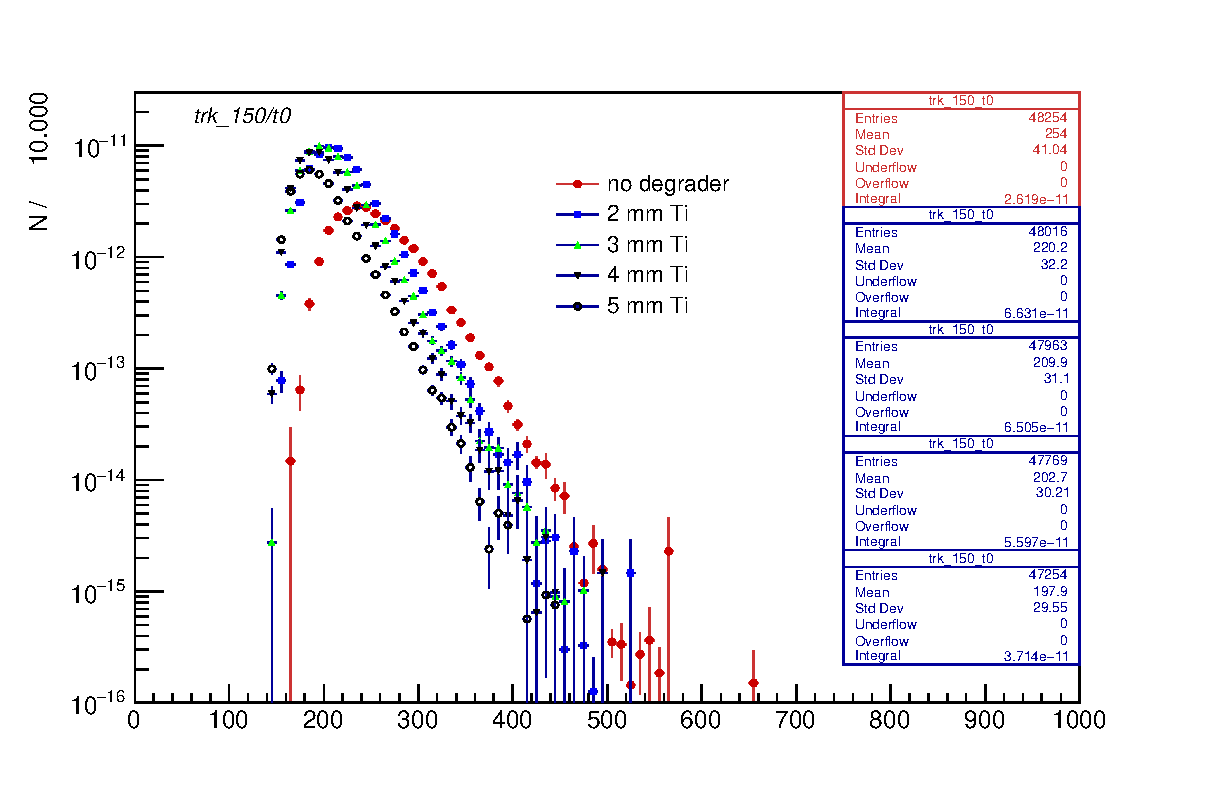
\includegraphics[width = 0.55\linewidth]{pdf/figure_00001}
  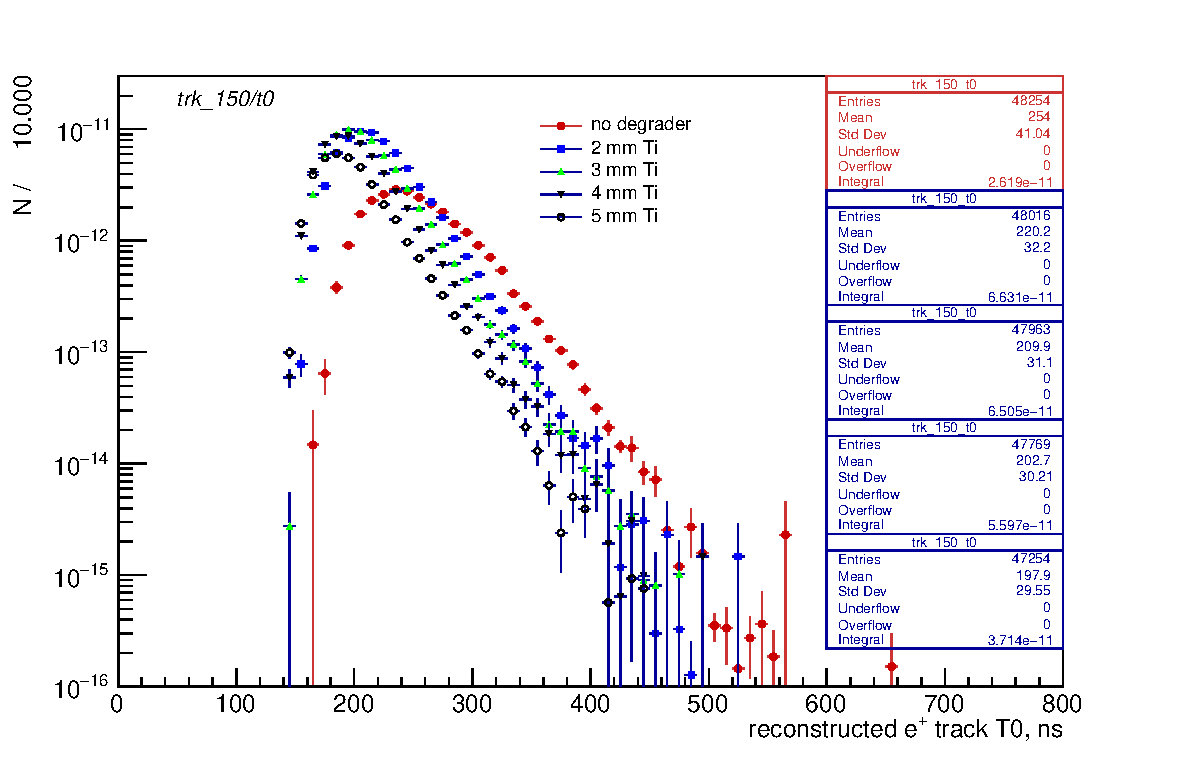
\includegraphics[width = 0.55\linewidth]{pdf/figure_00002}
  \caption{
    \label{fig:all_tracks_p_t0}
    Distributions of the reconstructed ST $\pi^+ \to e^+ \nu$ track momentum and time
    for different degrader thicknesses
  }
\end{figure}

%%%%%%%%%%%%%%%%%%%%%%%%%%%%%%%%%%%%%%%%%%%%%%%%%%%%%%%%%%%%%%%%%%%%%%%%%%%%%%
\subsection{Track selection cuts}

Based on the distributions in the track ID variables presented in Figure~\ref{fig:tid_variables_2mm},
we adopt the track ID cuts shown in the Table~\ref{table:track_id_cuts}

The cut values are very close to an old set of cuts known as "Set C" \cite{MU2E:3996:CutsetC}
and used by previous analyses, so a similar selection efficiency should be expected.

Cuts on $\tan \lambda$ and the track $d0$ provide significant rejection of the DIF
and $\pi \to e \nu$ decays in the degrader.

\begin{figure}[H]
  % \centering
  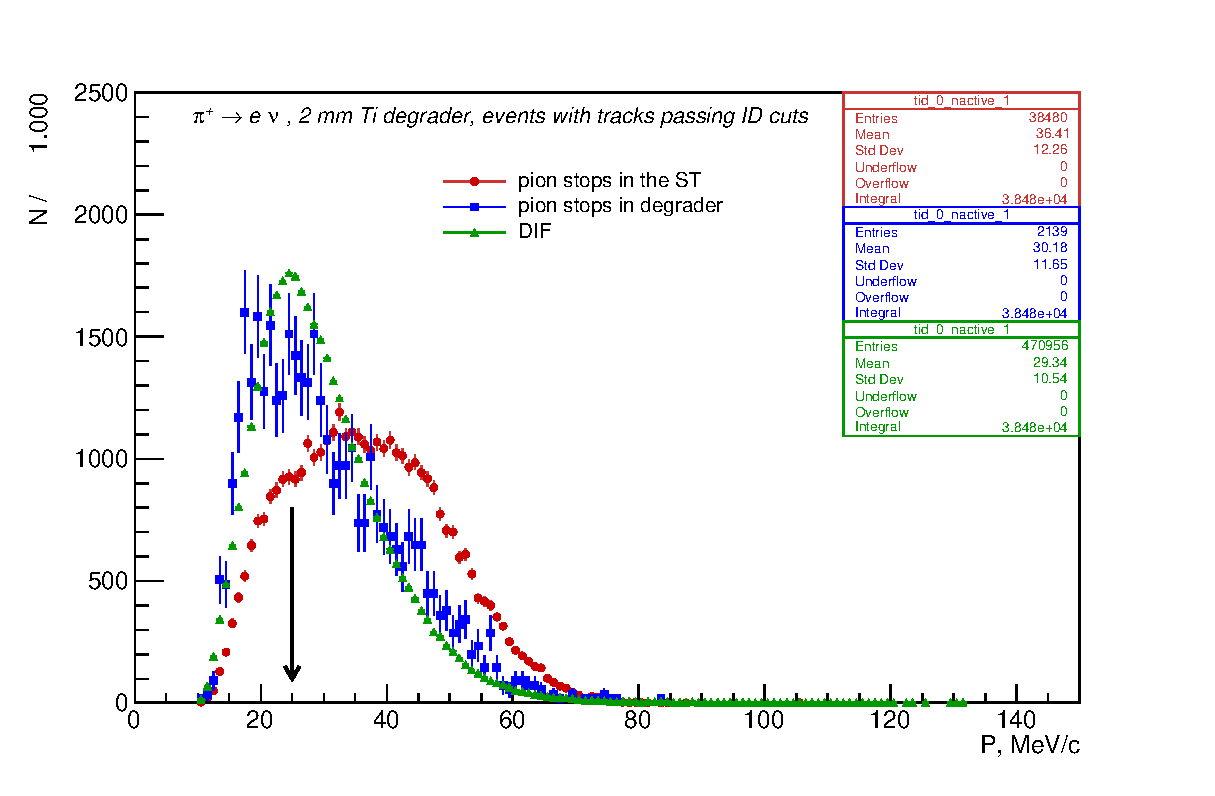
\includegraphics[width=0.55\linewidth]{pdf/figure_00274}  % tid_0/nactive_1
  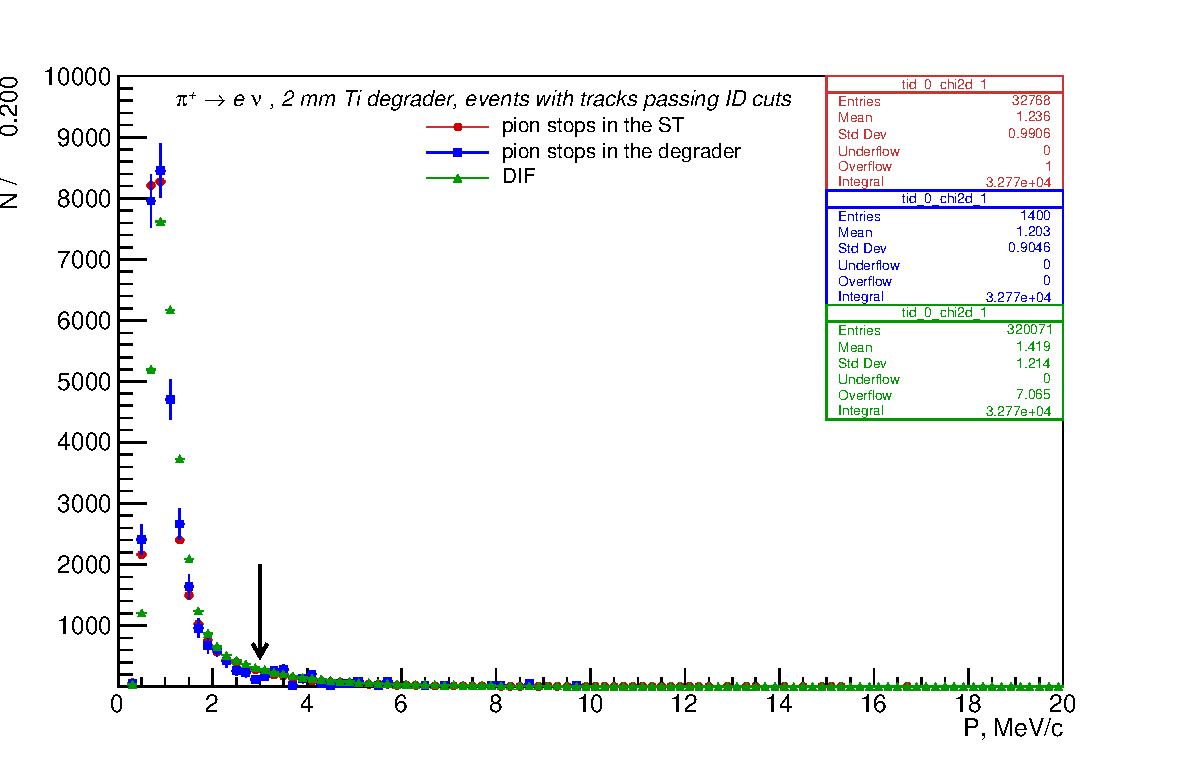
\includegraphics[width=0.55\linewidth]{pdf/figure_00275}  % tid_0/chi2d_1
  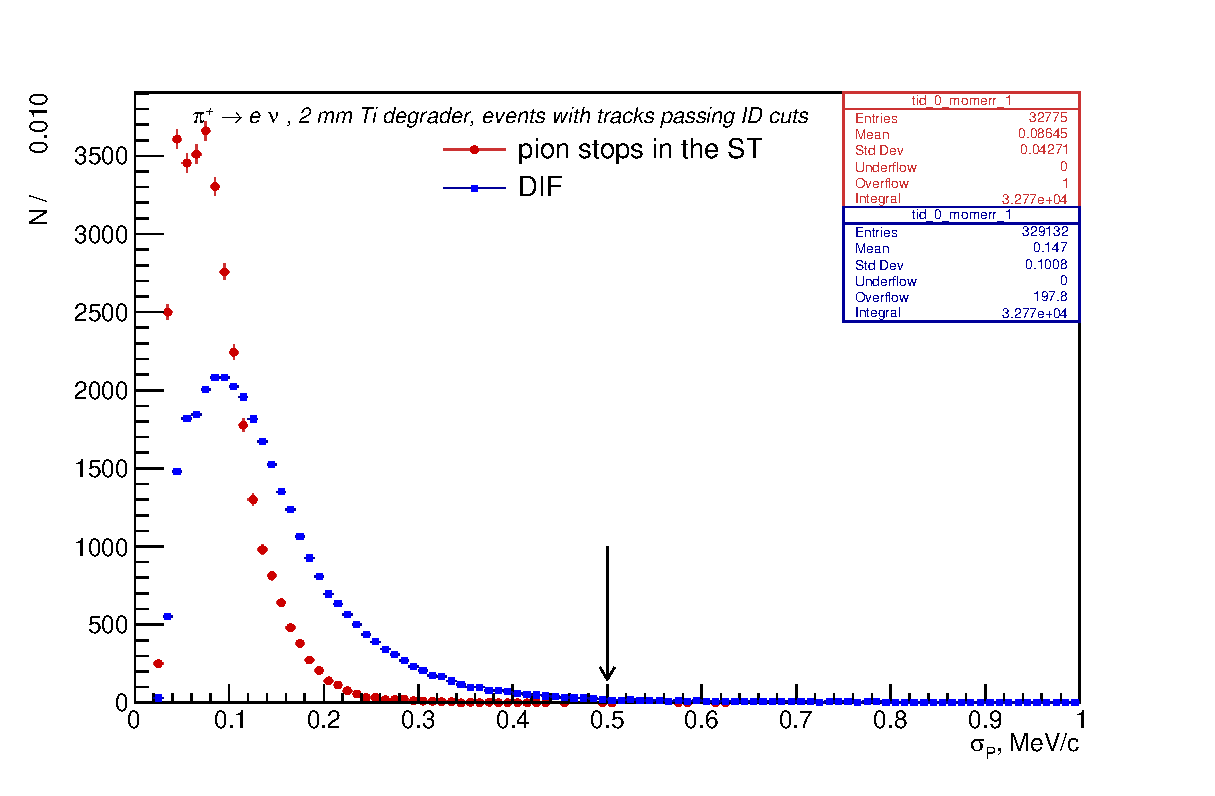
\includegraphics[width=0.55\linewidth]{pdf/figure_00276}  % tid_0/momerr_1
  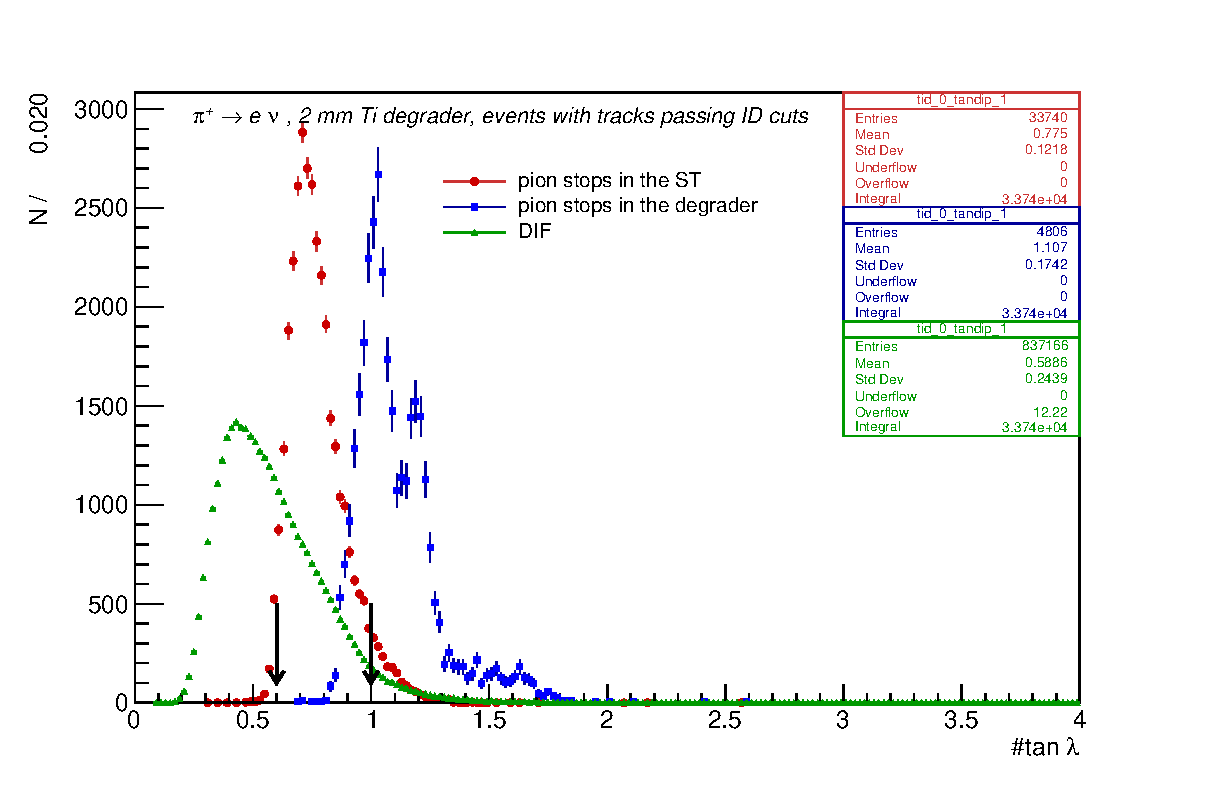
\includegraphics[width=0.55\linewidth]{pdf/figure_00273}  % tid_0/tandip_1
  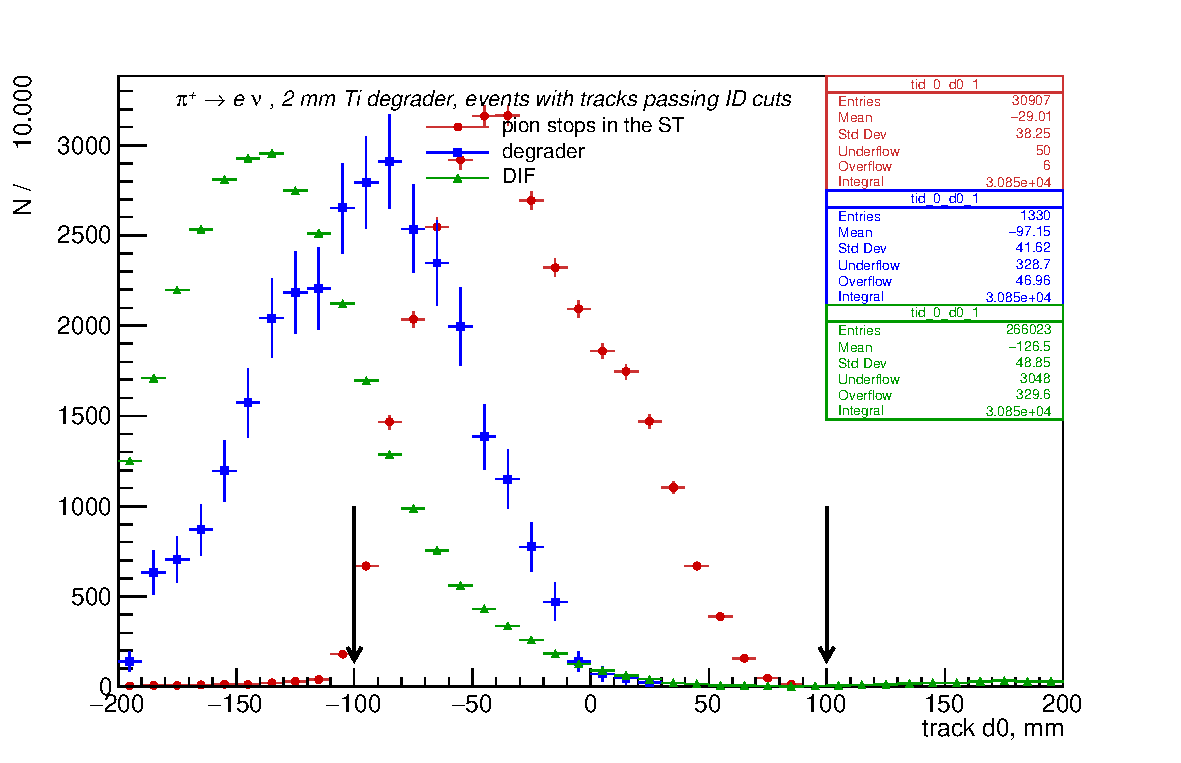
\includegraphics[width=0.55\linewidth]{pdf/figure_00277}  % tid_0/d0_1
  \caption{
    \label{fig:tid_variables_2mm}
    Distributions of the track ID variables for the 2mm Ti degrader
  }
\end{figure}

\begin{table}[H]
  \centering
  \begin{tabularx} {0.5\textwidth}{|X|c|}  %
    \hline
    variable                &   cut                        \\
    \hline                         
    N hits used by the fit  &   $N_{active}>= 25$            \\
    \hline                         
    chi2/DOF                &   $\chi2/DOF < 3$            \\
    \hline                         
    track dip angle         &   $0.6 < \tan \lambda < 1.0$ \\
    \hline                         
    track momentum error    &   $\sigma_P < 0.25$ MeV/c     \\
    \hline                         
    track $d_0$             &   $-100 < d_0 < 100$ mm     \\
    \hline
  \end{tabularx}
  \caption{
    \label{table:track_id_cuts}
    Track ID cuts
  }
\end{table}

It is worth noticing that the cut on the track dip angle significantly reduces
the contribution of positrons coming from $\pi^+ \to e^+ \nu$ decays in the degrader.

%%%%%%%%%%%%%%%%%%%%%%%%%%%%%%%%%%%%%%%%%%%%%%%%%%%%%%%%%%%%%%%%%%%%%%%%%%%%%%
\subsection{Signal reconstruction efficiency}

%% to see the number of entries and the weight, plot murat_pipenu_ana:trk_150/p_2

As shown in Table~\ref{table:reconstruction_eff}, the probability to reconstruct
a positron track from \piplusenu\ decay
is slightly below 50\% and it only marginally depends on teh thickness of the degrader.

\begin{table}[H]
\begin{tabularx}{1.0\textwidth} {|X|c|c|c|c|c|}  %
% \begin{tabular}{1.0\textwidth} {|l|l|}  %
  \hline
 degrader thickness &   Dataset  & probability for       &N $\pi^+$&N simulated  &N(reco tracks)     \\
 (mm)               &            & $\pi^+$ to stop in ST & stops   & \piplusenu\ &    ST             \\
  \hline                                                                                  
  no degrader       &   bpip0b0  &   4.23e-07            &  312616 &  100000     &   48254           \\
  \hline                                                                                  
     2              &   bpip2b0  &   1.11e-06            &   84785 &  100000     &   48016          \\
  \hline                                                                                  
     3              &   bpip3b0  &   1.09e-06            &   50340 &  100000     &  47963           \\
  \hline                                                                                  
     4              &   bpip4b0  &   9.44e-07            &   31681 &  100000     &  47769           \\
  \hline                                                                                  
     5              &   bpip5b0  &   6.35e-07            &   17225 &  100000     &  47254            \\
  \hline
\end{tabularx}
  \caption{
    \label{table:reconstruction_eff}
    Number of the events with reconstructed tracks for different pion datasets
  }
\end{table}

%%%%%%%%%%%%%%%%%%%%%%%%%%%%%%%%%%%%%%%%%%%%%%%%%%%%%%%%%%%%%%%%%%%%%%%%%%%%%%
\newpage
\subsection{Decays of pions stopped in the degrader}

Momentum distributions for reconstructed positron tracks from $\pi^+ \to e^+ \nu$ decays
in the ST and degrader are shown in Figure~\ref{fig:stt_vs_deg_momentum_good_tracks}.
The tracks are required to pass the selection cuts listed in Table~\ref{table:track_id_cuts}.
The selection efficiency is slightly higher than 60\%.

%%%%%%%%%%%%%%%%%%%%%%%%%%%%%%%%%%%%%%%%%%%%%%%%%%%%%%%%%%%%%%%%%%%%%%%%%%%%%%%
% before the selections cuts - all tracks - don't need
%%%%%%%%%%%%%%%%%%%%%%%%%%%%%%%%%%%%%%%%%%%%%%%%%%%%%%%%%%%%%%%%%%%%%%%%%%%%%%%
% \begin{figure}[H]
%   % \centering
%   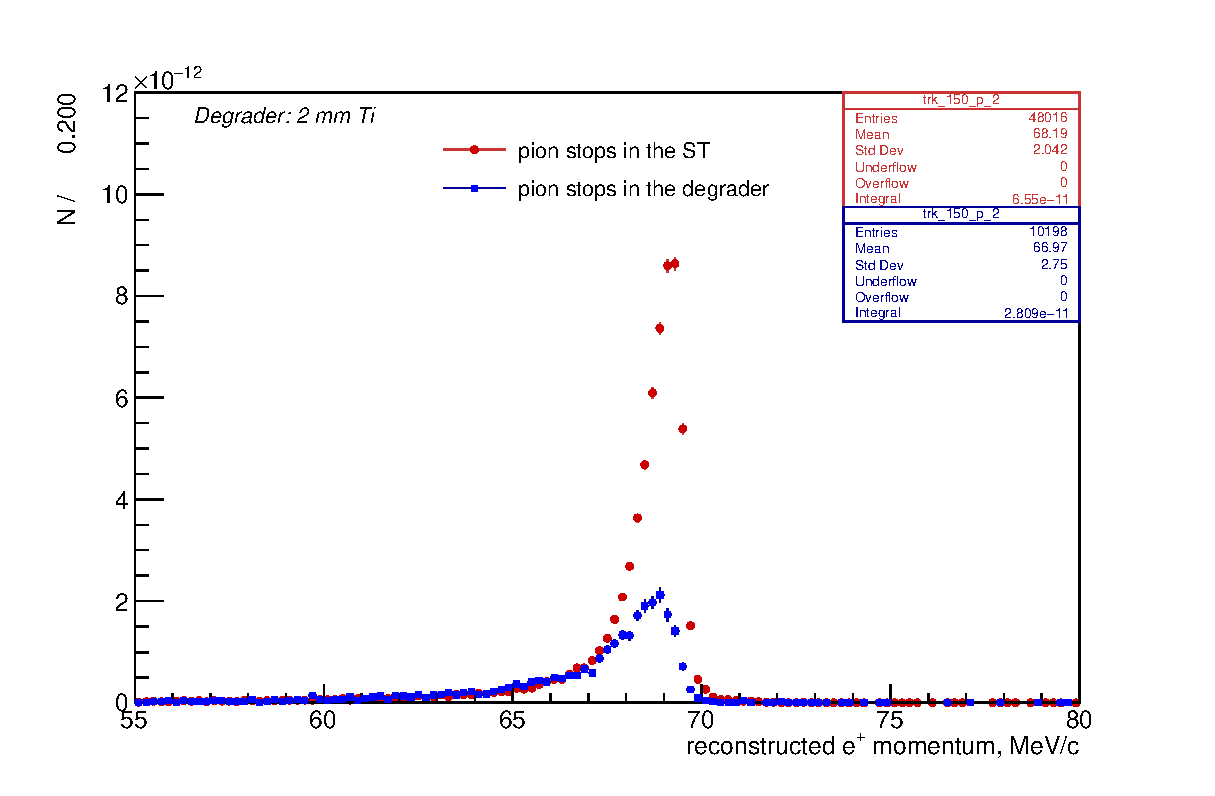
\includegraphics[width=0.55\linewidth]{pdf/figure_00251}
%   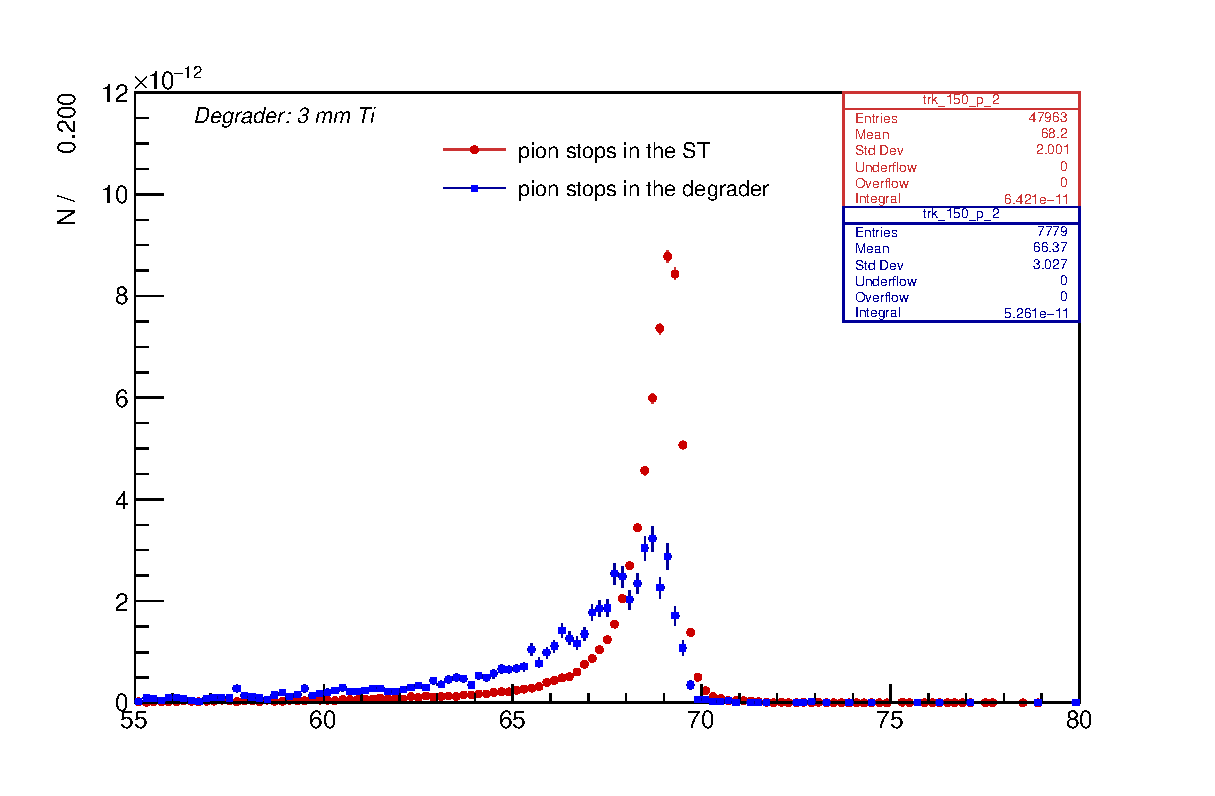
\includegraphics[width=0.55\linewidth]{pdf/figure_00351}
%   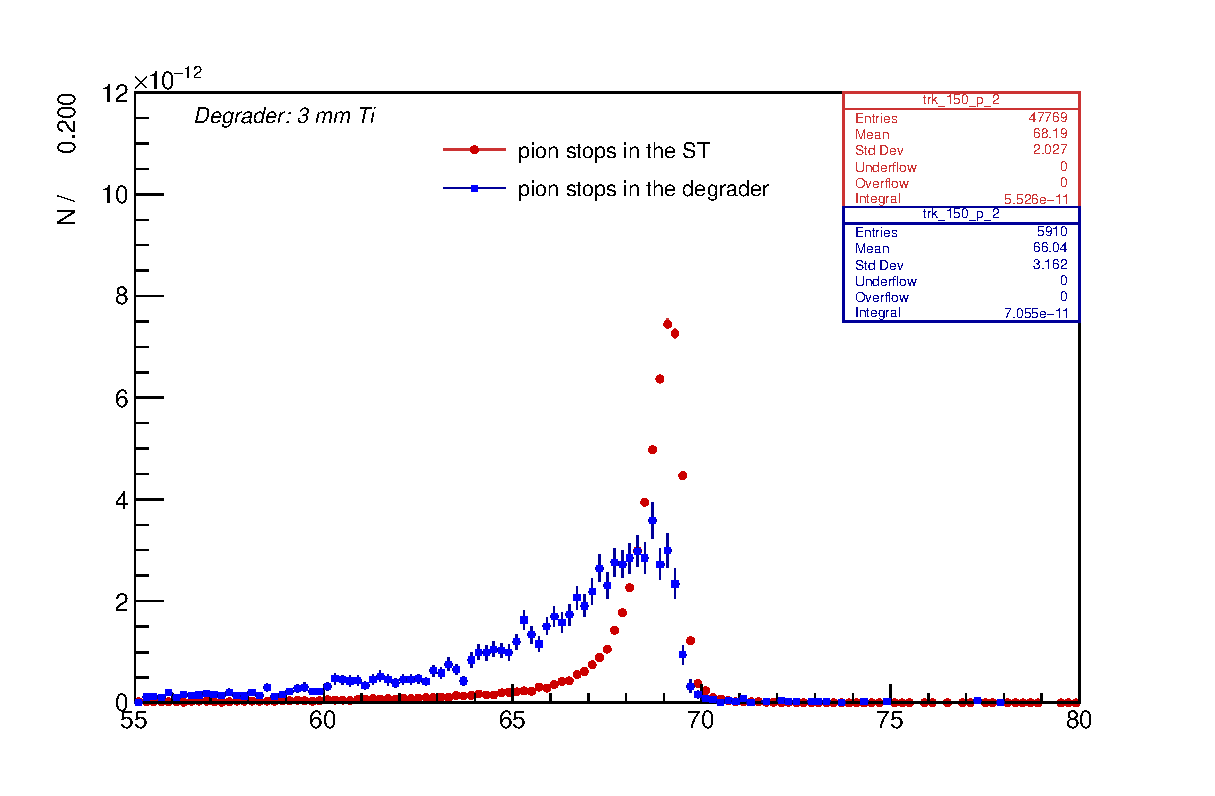
\includegraphics[width=0.55\linewidth]{pdf/figure_00451}
%   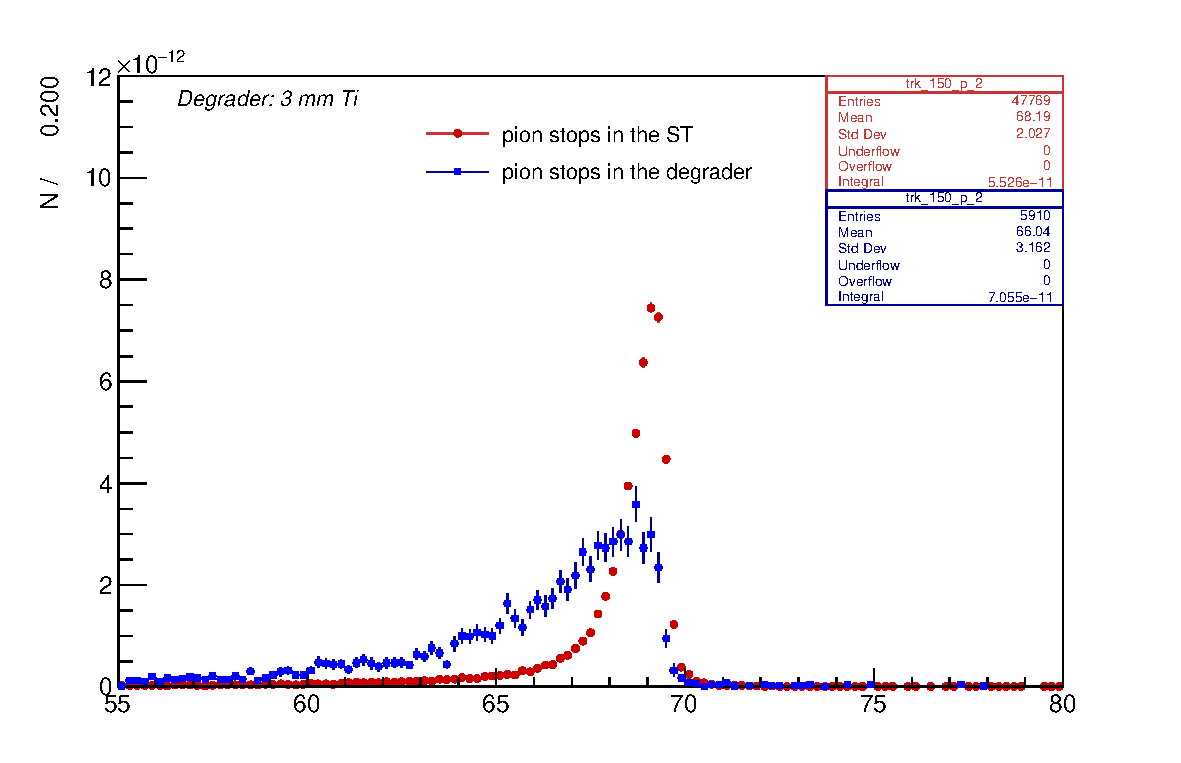
\includegraphics[width=0.55\linewidth]{pdf/figure_00551}
%   \caption{
%     % \label{fig:deg_vs_no_degrader_time}
%   }
% \end{figure}

\begin{figure}[H]
  % \centering
  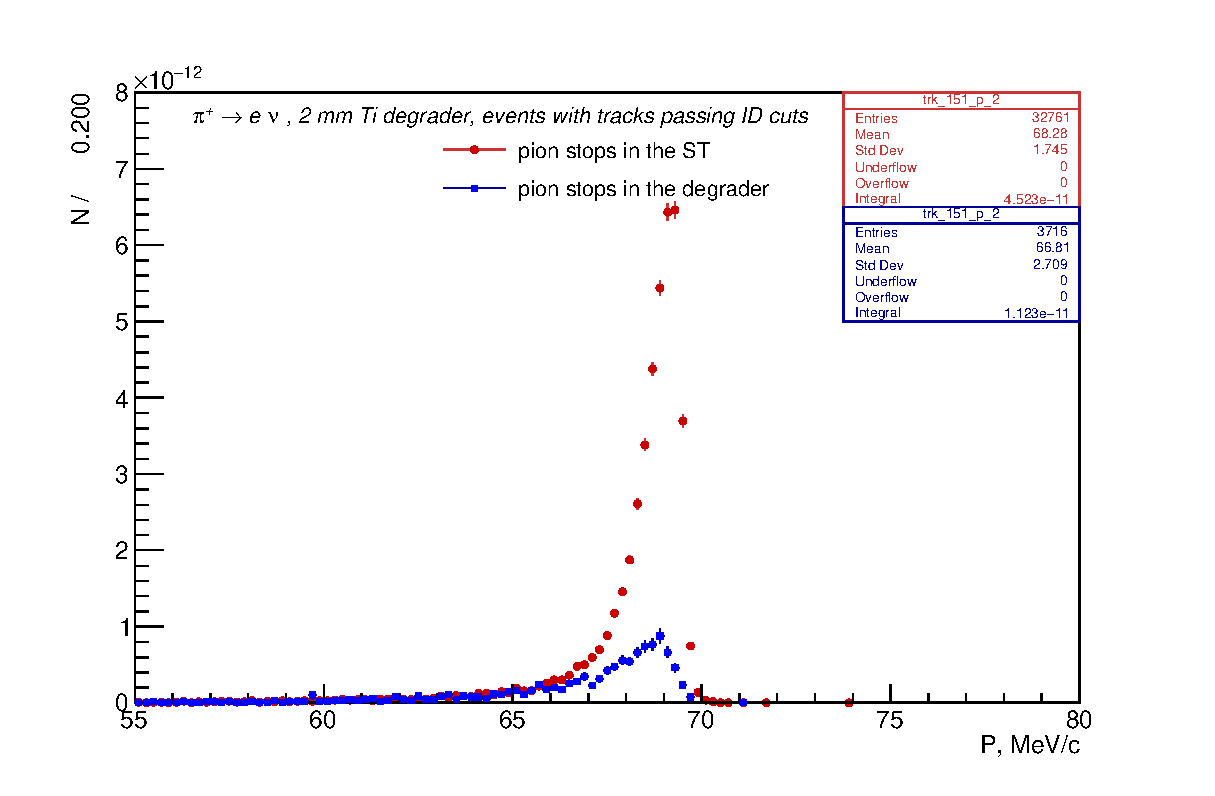
\includegraphics[width=0.55\linewidth]{pdf/figure_00261}
  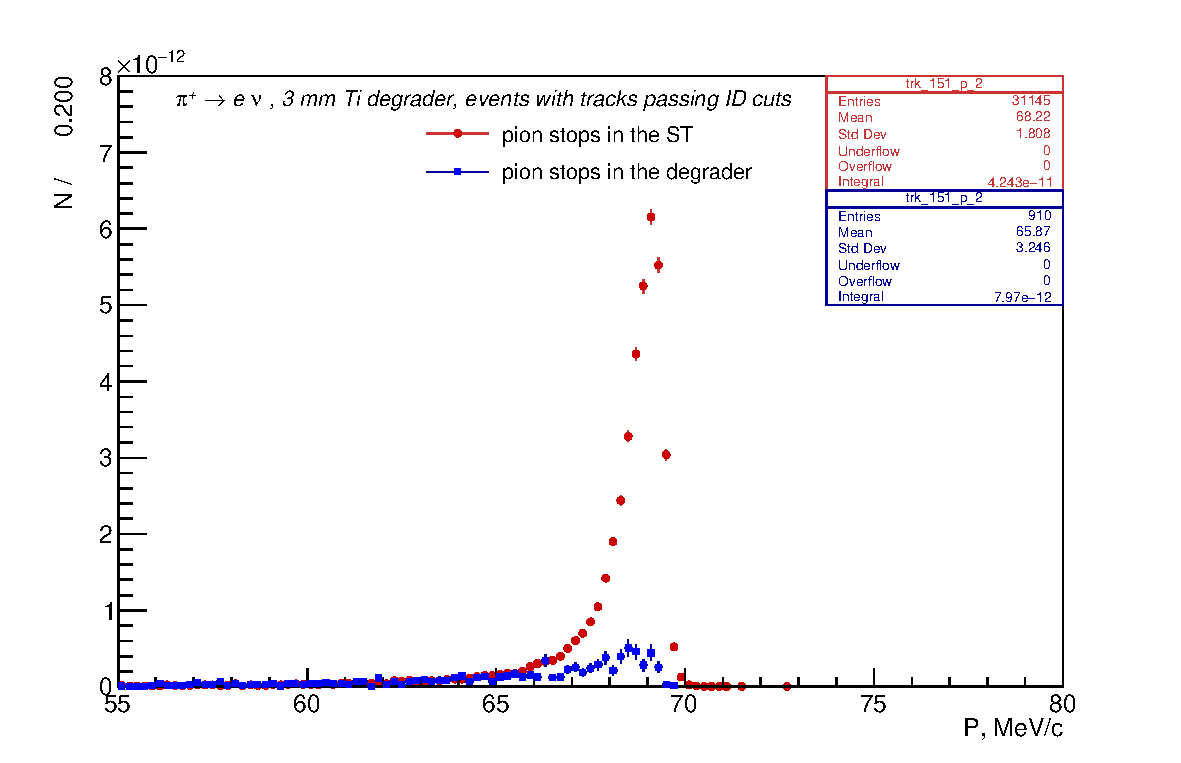
\includegraphics[width=0.55\linewidth]{pdf/figure_00361}
  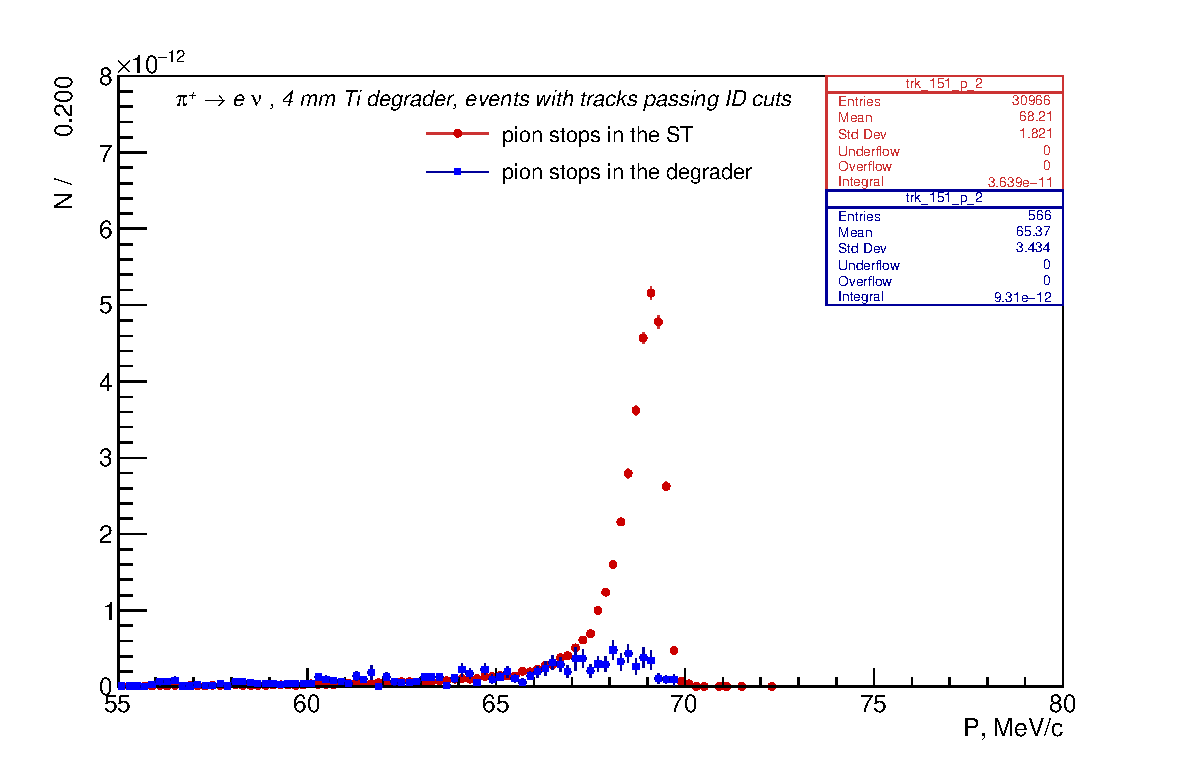
\includegraphics[width=0.55\linewidth]{pdf/figure_00461}
  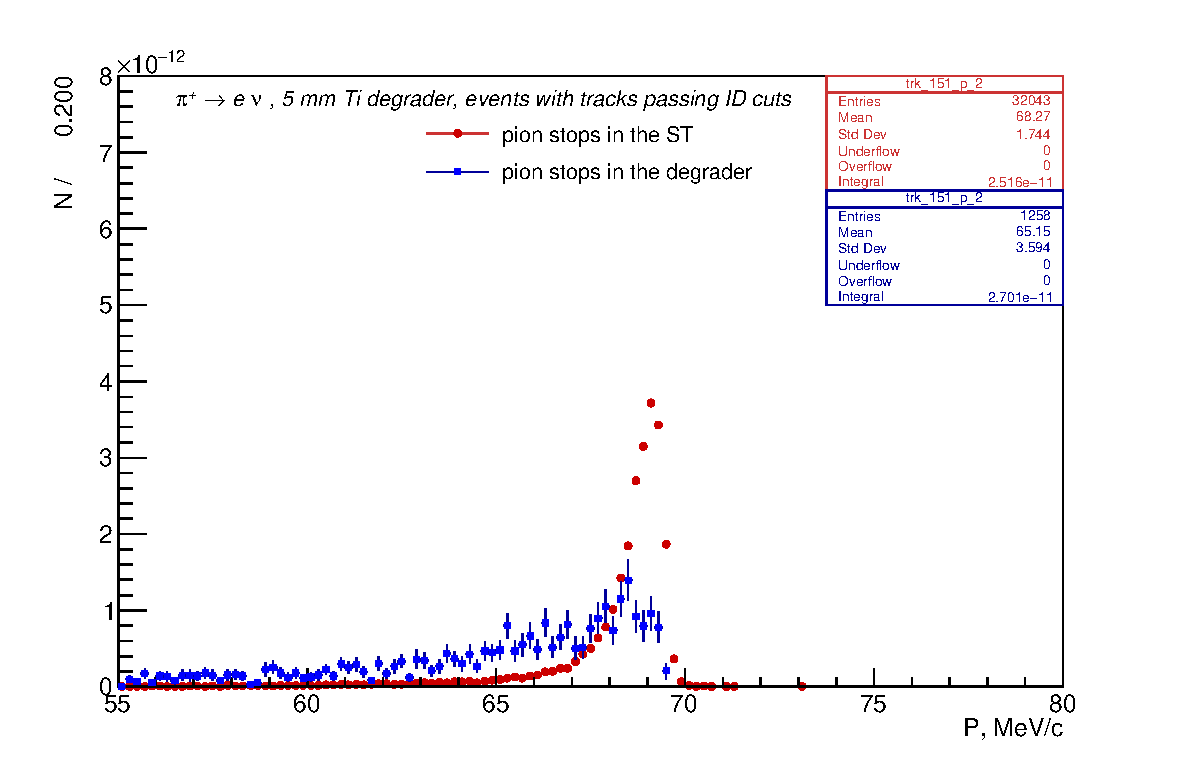
\includegraphics[width=0.55\linewidth]{pdf/figure_00561}
  \caption{
    \label{fig:stt_vs_deg_momentum_good_tracks}
    reconstructed e+ yield/POT for different degrader thicknesses, STT vs DEG
  }
\end{figure}

For the signal window $67.5 < P < 70$ MeV/c, the relative contribution of pion
decays in degrader is in the range of 10-15\%.

Timing distributions for tracks from \piplusenu\ decays in the ST and degrader and
passing the selection cuts are shown if Figure~\ref{figure:stt_vs_deg_t0_good_tracks}.
As, on average, slower pions stop in the degrader, the timing distributions 
of decays in the degrader fall a little bit slower.
Therefore, at large T0 the contribution of the degrader stops increases.


\begin{figure}[H]
  % \centering
  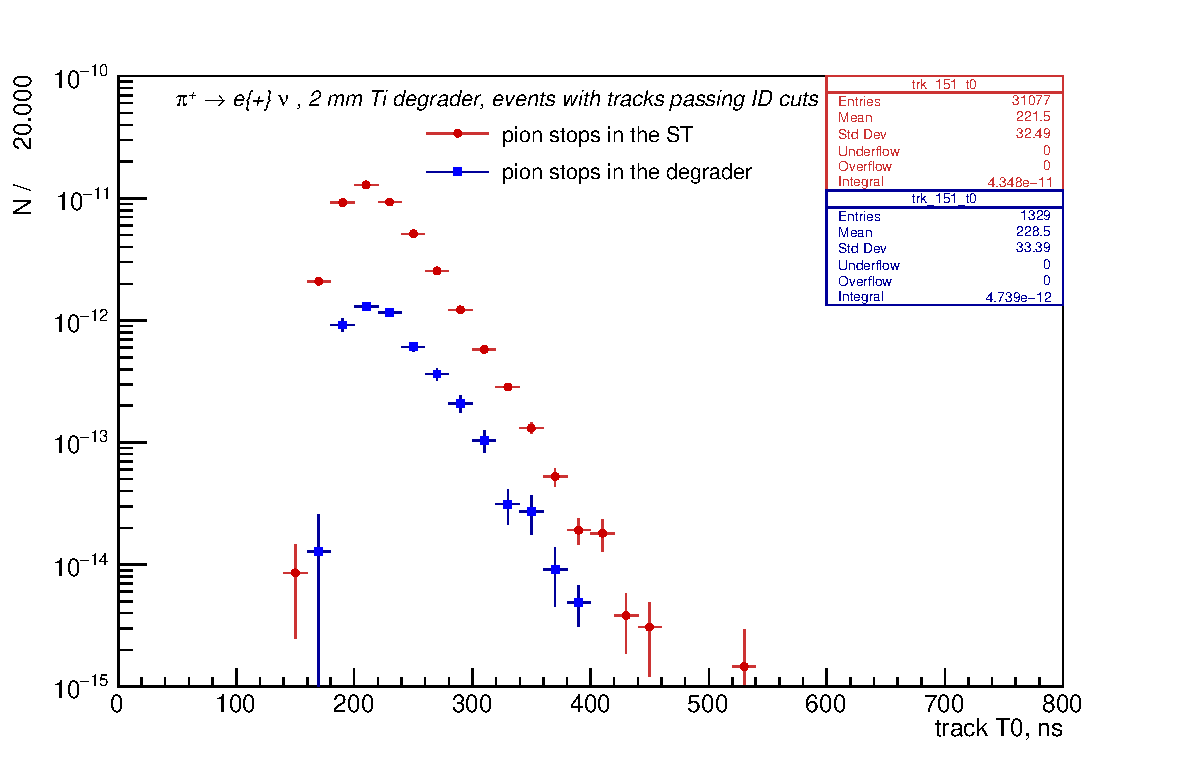
\includegraphics[width=0.55\linewidth]{pdf/figure_00262}
  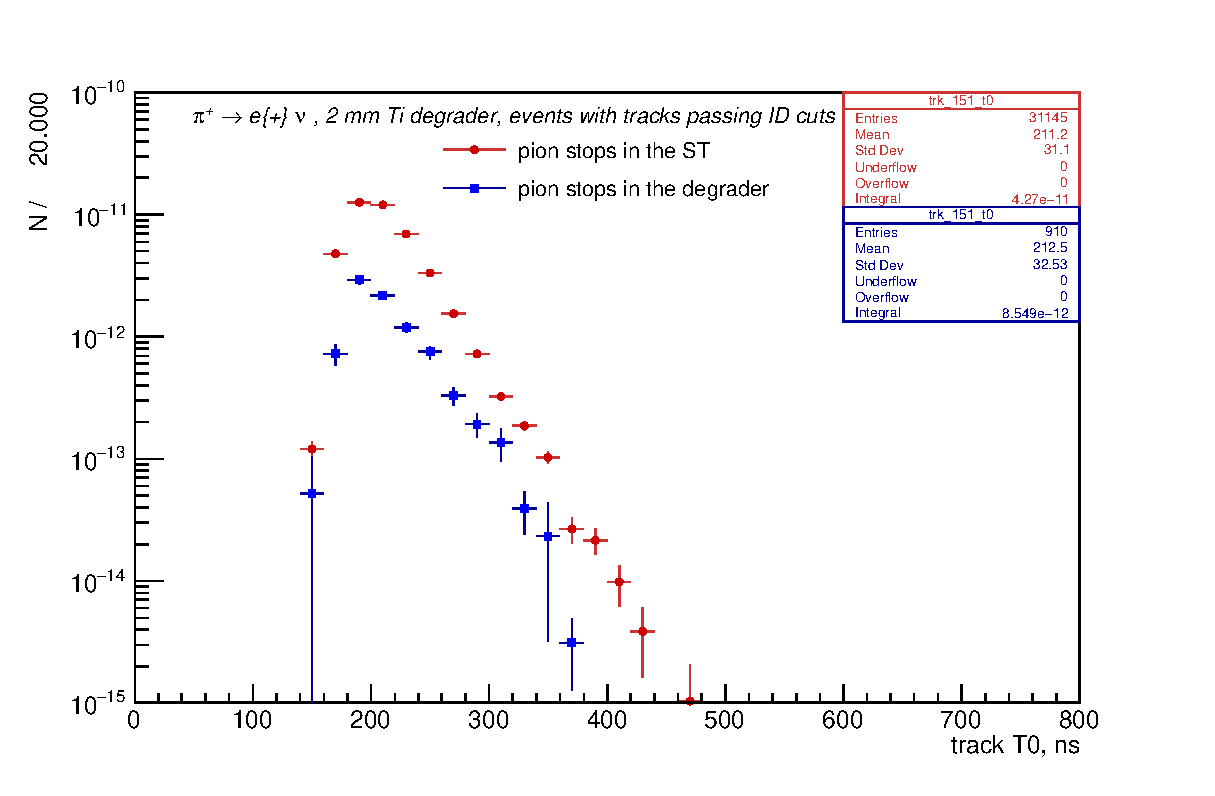
\includegraphics[width=0.55\linewidth]{pdf/figure_00362}
  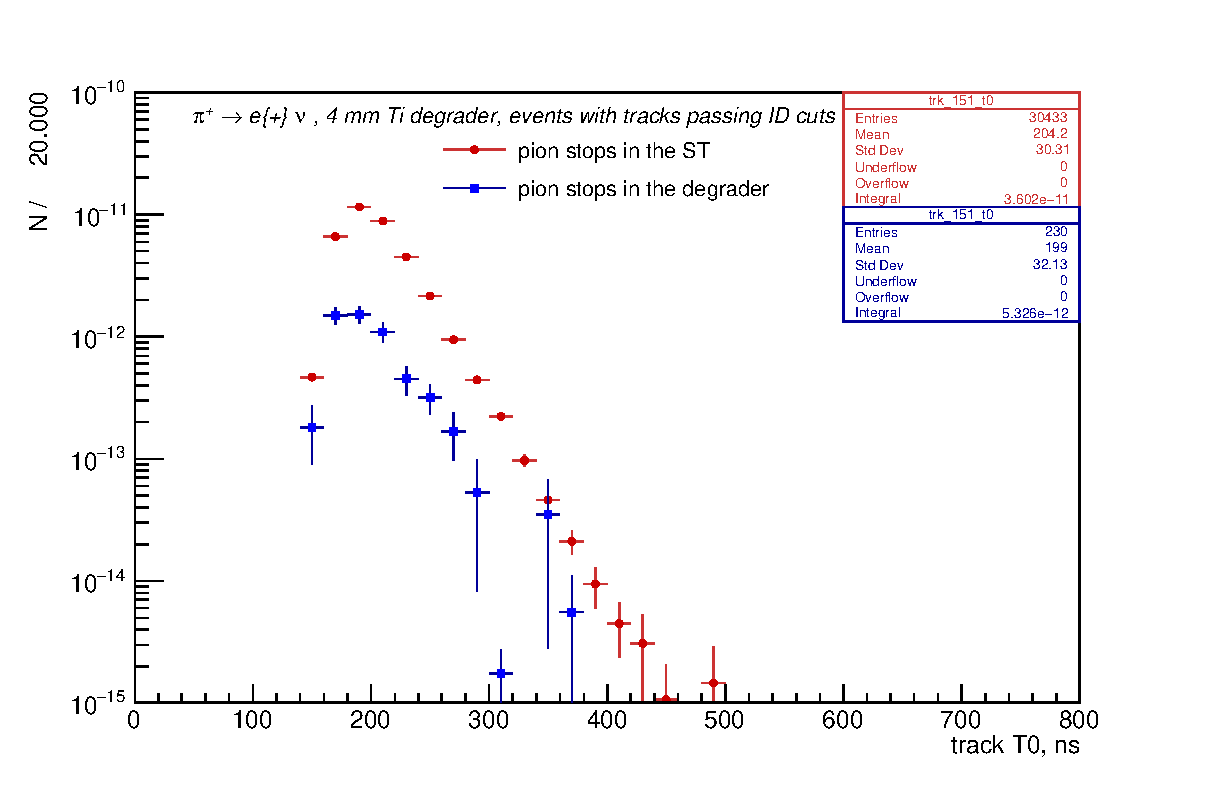
\includegraphics[width=0.55\linewidth]{pdf/figure_00462}
  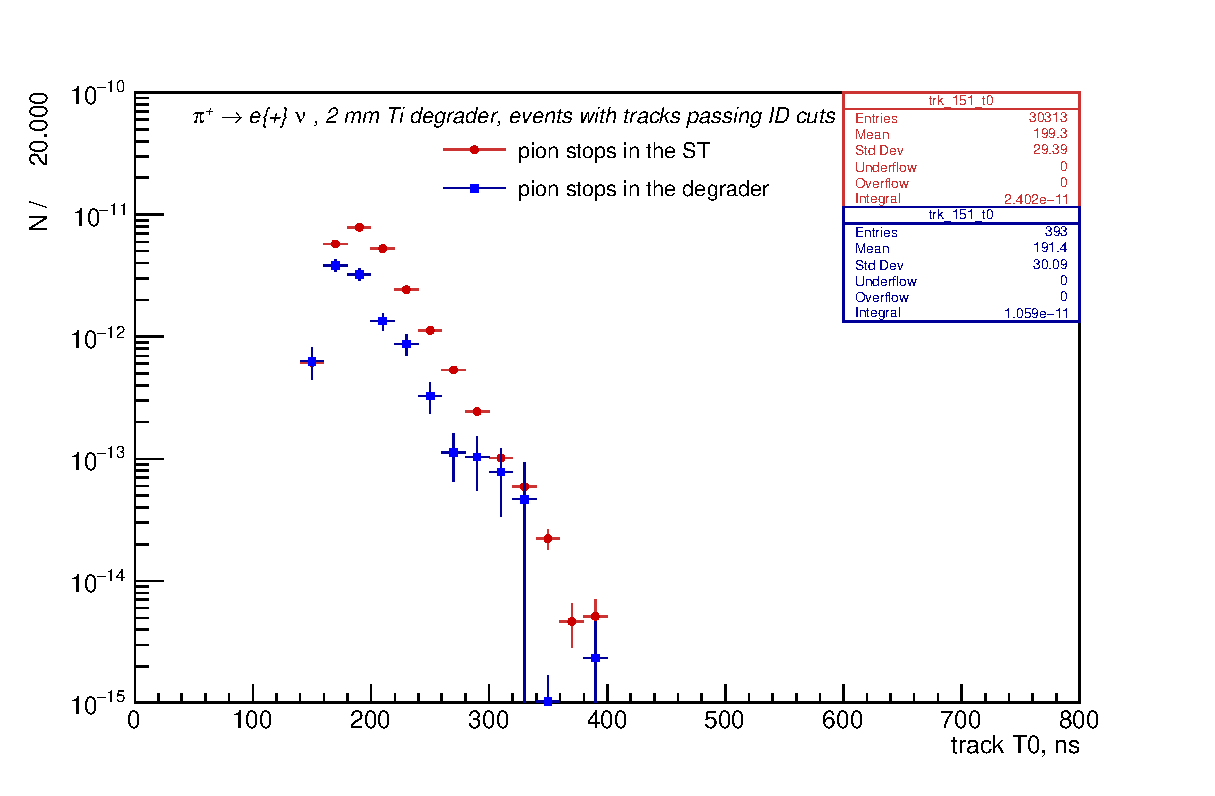
\includegraphics[width=0.55\linewidth]{pdf/figure_00562}
  \caption{
    \label{figure:stt_vs_deg_t0_good_tracks}
    reconstructed e+ yield/POT for different degrader thicknesses, STT vs DEG
  }
\end{figure}

%%%%%%%%%%%%%%%%%%%%%%%%%%%%%%%%%%%%%%%%%%%%%%%%%%%%%%%%%%%%%%%%%%%%%%%%%%%%%%
\subsection{Standard selection - results}

Figure~\ref{figure:no_deg_mom} shows momentum distributions of reconstructed
positron tracks from positive pion decays in the ST and muon decays in flight
for the detector configuration w/o the degrader. 
The tracks are required to pass the selection cuts and have the T0 > 300 ns. 
The \piplusenu\ signal is expected to be buried deep under the DIF background.

\begin{figure}[H]
  % \centering
  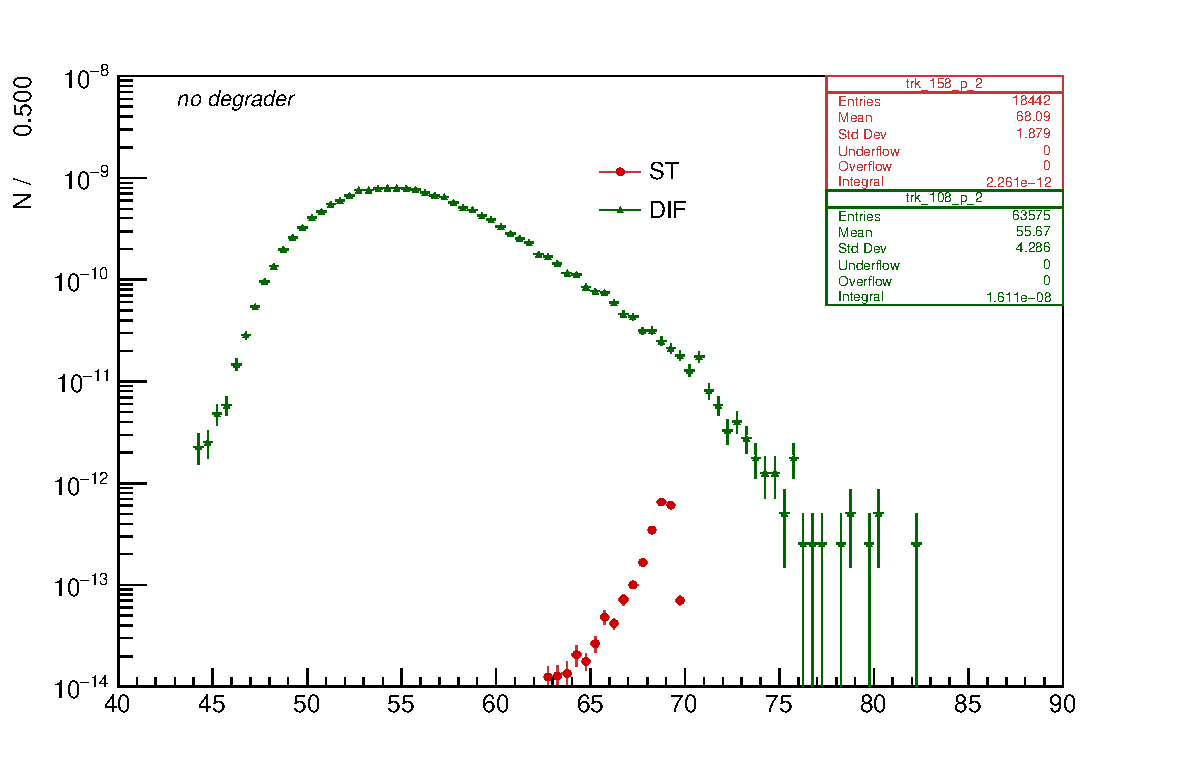
\includegraphics[width=0.90\linewidth]{pdf/figure_00031}
  \caption{
    \label{figure:no_deg_mom}
  }
\end{figure}

Distributions for different degrader thicknesses after T0>300 ns cut are shown
in Figure~\ref{figure:deg_mom}

\begin{figure}[H]
  % \centering
  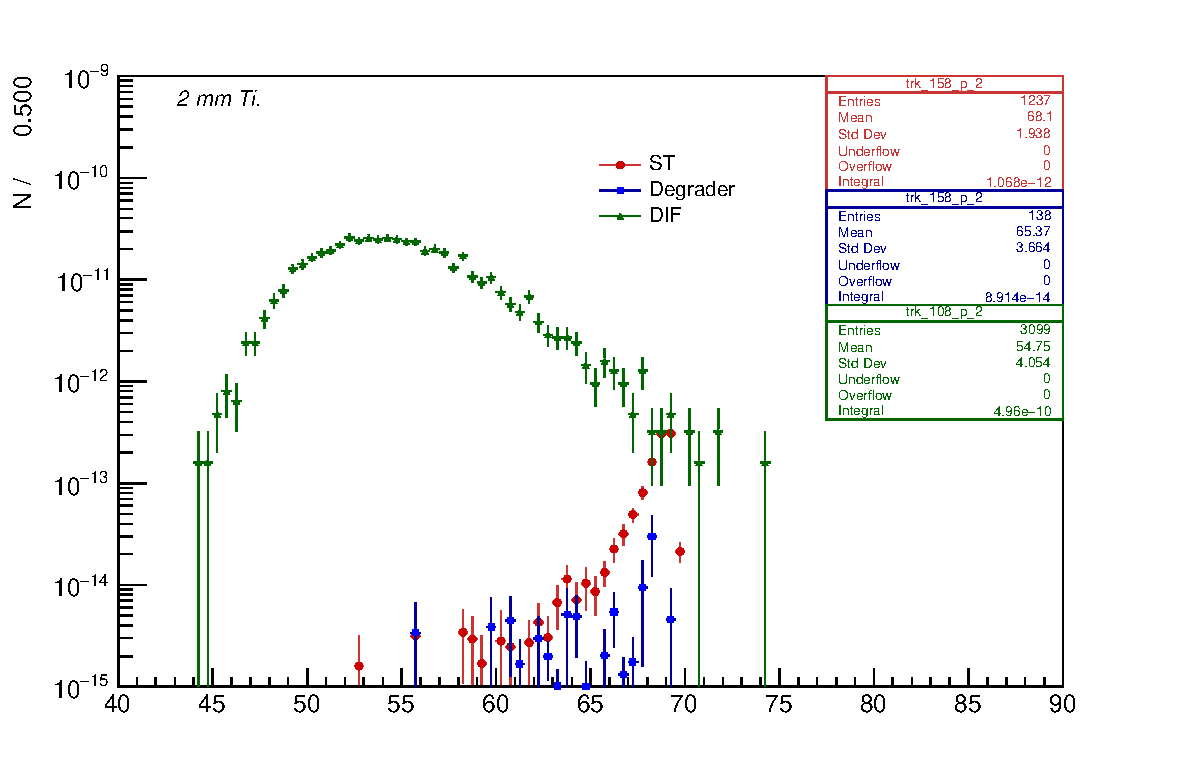
\includegraphics[width=0.55\linewidth]{pdf/figure_00231}
  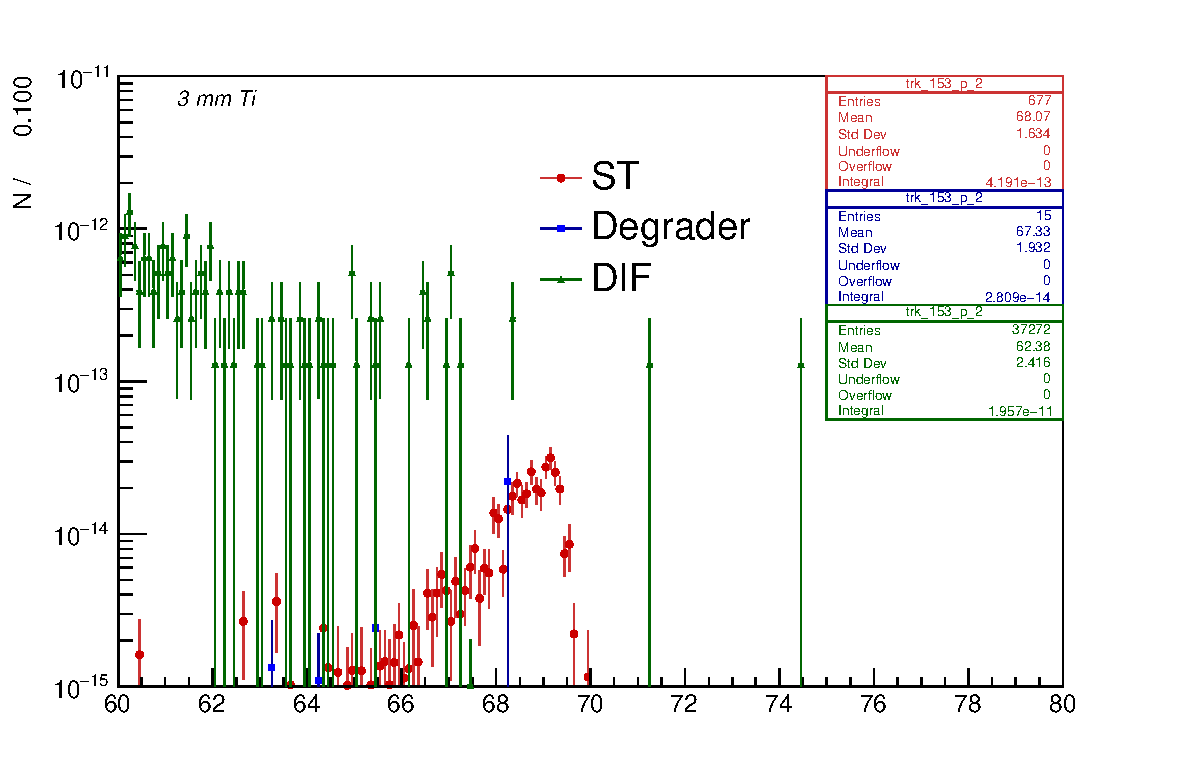
\includegraphics[width=0.55\linewidth]{pdf/figure_00331}
  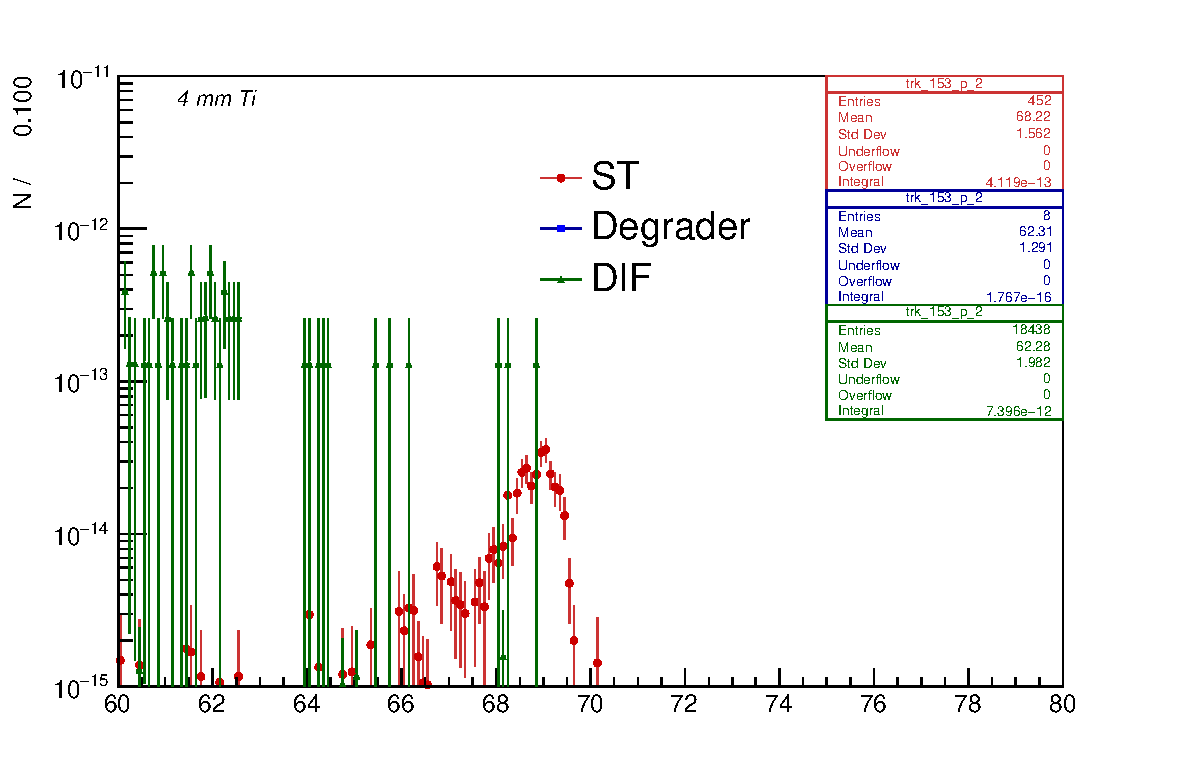
\includegraphics[width=0.55\linewidth]{pdf/figure_00431}
  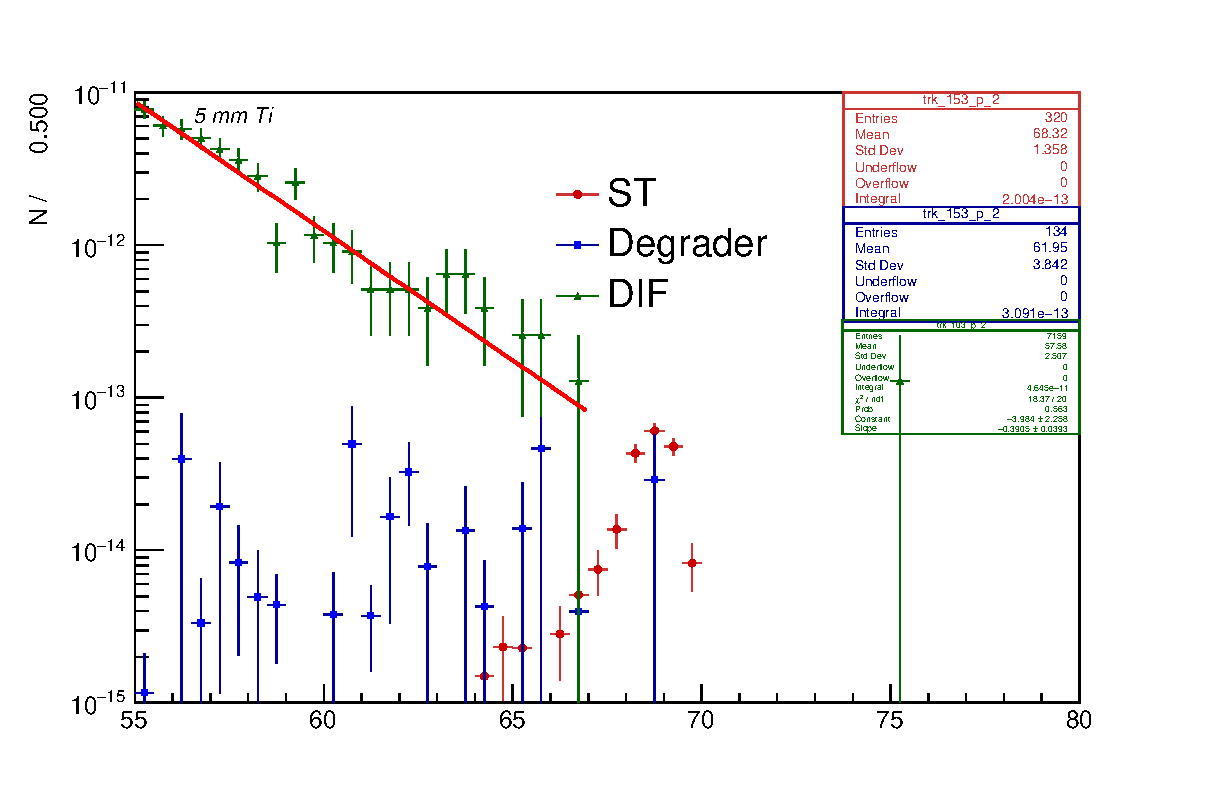
\includegraphics[width=0.55\linewidth]{pdf/figure_00531}
  \caption{
    \label{figure:deg_mom}
  }
\end{figure}

The signal vs background situation looks more promising, however thre is no clear indication
that the \piplusenu\ signal would be clearly seen on top of the DIF background.
The plots also do not indicate that increasing the degrader thickness from 2mm to 5mm 
improves  the signal to background ratio (S/B) in any significant way - the available
statistics is not sufficient for drawing such a conclusion.

For degrader thickness of 4mm, a visual scan of DIF events surviving
the selection cuts and having  hte reconstructed positron momentum above 65 MeV/c
has been performed.
%
The surviving events are dominated by correctly reconstructed events on the high-momentum tail
of the $\mu^+$ decays-in flight spectrum, and not by mis-reconstructed events.

%%% Local Variables:
%%% mode: latex
%%% TeX-master: "mu2e-xxxxx"
%%% End:
